\chapter{Математическая модель переноса излучения}
Одним из способов описать поле излучения является классический статистический подход на основании функции распределения световых квантов. Пусть $f(\nu, \vec r, \vec \Omega) d\nu d\vec r d\vec \Omega$ есть число фотонов в спектральном диапазоне $[\nu, \nu+d\nu]$, находящихся в момент времени $t$ в элементе объёма $d\vec r$ в окрестности точки $\vec r$ и имеющих направление движения в элементе телесного угла $d\vec\Omega$ около единичного вектора $\vec \Omega$. С данной функцией распределения можно связать спектральную интенсивность излучения
\[
I_\nu(\vec r, \vec \Omega, t) = h\nu c f(\nu, \vec r, \vec \Omega, t).
\]
Величина $I_\nu d\nu d\vec \Omega$ определяет количество лучистой энергии в спектральном интервале $[\nu, \nu + d\nu]$, протекающей в $1$ сек через площадку в $1 \text{ см}^2$, расположенную в точке $\vec r$ нормально к направлению распространения квантов, расположенном в элементе телесного угла $d\vec \Omega$ около вектора $\vec \Omega$. Задание функций $f$ или $I_\nu$ однозначно определяет поле излучения.

Спектральной плотностью излучения $U_\nu$ называется
\[
U_\nu(\vec r, t) = \frac{1}{c}\int\limits_{4\pi} I_\nu(\vec r, \vec \Omega, t) d\Omega.
\]
Количество лучистой энергии, заключенной в элементарном объёме $d\vec r$ в интервале частот $[\nu, \nu + d\nu]$ соответствует $U_\nu(\vec r, t) d\nu d\vec r$. Вектором спектральной плотности потока энергии излучения, или вектором Пойтинга, называется
\[
\vec S_\nu = \int\limits_{4\pi} I_\nu \vec \Omega d\Omega.
\]
Полные интенсивность, плотность и поток энергии излучения получаются из соответствующих спектральных величин интегрированием по всему спектру:
\[
I = \int_0^\infty I_\nu d\nu, \qquad
U = \int_0^\infty U_\nu d\nu, \qquad
\vec S = \int_0^\infty \vec S_\nu d\nu.
\]

\section{Уравнение переноса излучения}

В данной работе сделан ряд предположений о процессе переноса излучения:
\begin{itemize}
\item пренебрегается нестационарностью процесса переноса излучения;
\item не учитывается рассеяние излучения с изменением направления полета фотонов;
\item не учитываются эффекты, приводящие к изменению частоты излучения.
\end{itemize}
При данных предположениях для интенсивности излучения $I_\nu(\vec r, \vec \Omega)$ справедливо уравнение \cite{zeldovich2008}:
\begin{equation}
(\vec \Omega \nabla) I_\nu(\vec r, \vec \Omega) + \varkappa_\nu(\vec r, \vec \Omega) I_\nu(\vec r, \vec \Omega) = 
\varkappa_\nu(\vec r, \vec \Omega) I_{\nu,\text{p}}(\vec r, \vec \Omega),
\label{eq:transfer}
\end{equation}
где $\varkappa_\nu$ --- коэффициент поглощения излучения, исправленный на вынужденное испускание, $I_{\nu, \text{p}}$ --- интенсивность равновесного излучения. Предполагается, что коэффициент поглощения и интенсивность равновесного излучения в точке $\vec r$ могут быть различным для различных направлений $\vec \Omega$. Это позволяет учитывать доплеровские сдвиги частоты поглощения и испускания в движущемся веществе. При этом скорость движения предполагается дорелятивистской, так как в противном случае предположение о стационарности процесса переноса излучения не выполняется. Данное уравнение выражает баланс лучистой энергии, заключенной в элементарном цилиндре, окружающем луч $\vec r - \vec r_0 = \vec \Omega s$.
%, см. рисунок \ref{fig:cyl}.
%\begin{figure}[ht!]
%\centering
%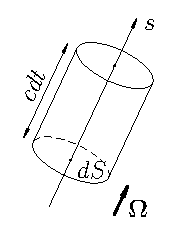
\includegraphics[height=.2\textheight]{radiation-0.eps}
%\caption{Элементарный цилиндр, окружающий луч $\vec r - \vec r_0 = \vec \Omega s$}
%\label{fig:cyl}
%\end{figure}

Для уравнения \eqref{eq:transfer} в ограниченной выпуклой области $G$ необходимо задать интенсивность $I_\nu$ на границе $\partial G$ для лучей, входящих в область. Если обозначить внешнюю нормаль к границе области $\partial G$ как $\vec n$, то граничное условие принимает вид
\[
I_\nu(\vec r, \vec \Omega) = I_{\nu,0}(\vec r, \vec \Omega), \quad \vec r \in \partial G,\; (\vec n \vec \Omega) < 0.
\]
При этом $I_{\nu,0}$ может быть
\begin{itemize}
\item нулем, в данном случае говорят об отсутствии источников излучения вне области $G$;
\item заданной известной функцией;
\item выраженной через интенсивность излучения, падающего на границу.
\end{itemize}
Последний тип условий наиболее сложный, но позволяет описывать отражение и рассеяние излучения границей области. Условия зеркального отражения имеют вид
\[
I(\vec r, \vec \Omega) = I(\vec r, \vec \Omega'), \quad \vec r \in \partial G, \; \vec \Omega' = \vec \Omega + 2 (\vec \Omega \vec n) \vec n,
\]
где $\vec \Omega'$ --- зеркальное отражение вектора $\vec \Omega$ относительно касательной плоскости.
% (см. рисунок \ref{fig:reflect})
%\begin{figure}[ht!]
%\centering
%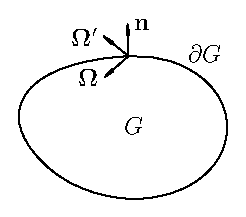
\includegraphics[height=.15\textheight]{radiation-1.eps}
%\caption{Зеркальное отражение излучения от границы}
%\label{fig:reflect}
%\end{figure}
В данной работе этот тип условий не рассматривается.

Довольно часто от уравнения \eqref{eq:transfer}, переходят к одночастотному уравнению, которое можно получить, усредняя уравнение в частотной группе $\nu \in [\nu_1, \nu_2]$. При этом делается предположение о том, что величина
\[
\varkappa = \frac{\int_{\nu_1}^{\nu_2} \varkappa_\nu(\vec r, \vec \Omega) I_\nu(\vec r, \vec \Omega) d\nu}{
\int_{\nu_1}^{\nu_2} I_\nu(\vec r, \vec \Omega) d\nu
}
\]
не зависит от интенсивности $I_\nu(\vec r, \vec \Omega)$, а определяется некоторым усреднением только коэффициента поглощения $\varkappa_\nu(\vec r, \vec \Omega)$. В качестве таких усреднений обычно применяют усреднение по Планку либо по Росселанду \cite{zeldovich2008}:
\begin{gather*}
\varkappa_\text{Планк} = \frac{\int_{\nu_1}^{\nu_2} \varkappa_\nu I_{\nu, \text{p}} d\nu}{\int_{\nu_1}^{\nu_2} I_{\nu, \text{p}} d\nu}\\
\varkappa_\text{Росселанд}^{-1} = \frac{\int_{\nu_1}^{\nu_2} \varkappa_\nu^{-1} \frac{dU_{\nu, \text{p}}}{dT} d\nu}{\int_{\nu_1}^{\nu_2} \frac{dU_{\nu, \text{p}}}{dT} d\nu}.
\end{gather*}
После осреднения по частоте уравнение переноса сохраняет свой вид, поэтому далее, если не указано обратное, рассматриваем одночастотное уравнение. Усреднение уравнения в наборе частотных групп $[\nu_i, \nu_{i+1}]$ называется многогрупповым приближением.

Необходимо отметить, что в системе уравнений радиационной газовой динамики роль излучения ограничивается добавочными слагаемыми в плотность и плотность потока импульса, а также в плотность и плотность потока энергии системы <<вещество + излучение>>. Система радиационной газовой динамики принимает вид \cite{chetverushkin1985}
\[
\begin{gathered}
\pd{\rho}{t} + \div \rho \vec u = 0\\
\pd{(\rho \vec u + \vec S / c^2)}{t} + \div \left(\rho \vec u \vec u + p \mathbb I + \mathbb T \right) = 0\\
\pd{(e + U)}{t} + \div \left((e + p)\vec u + \vec S \right) = 0\\
e = \rho \left(\varepsilon + \frac{u^2}{2}\right),\quad  p = p(\rho, \varepsilon).
\end{gathered}
\]
В данной системе $\mathbb T$ --- тензор потока импульса излучения, определенный как
\[
\mathbb T(\vec r) = \int\limits_0^\infty \mathbb T_\nu(\vec r) d\nu, \qquad
\mathbb T_\nu(\vec r) = \frac{1}{c}\int\limits_{4\pi} \vec \Omega \vec \Omega I_\nu(\vec r, \vec \Omega) d\Omega.
\]
Для большинства задач радиационной газовой динамики слагаемыми более низкого порядка по $c$ можно пренебречь. Так как $U,\mathbb T \sim c^{-1} I,\; \vec S \sim c^0 I$, система упрощается до
\[
\begin{gathered}
\pd{\rho}{t} + \div \rho \vec u = 0\\
\pd{\rho \vec u}{t} + \div \left(\rho \vec u \vec u + p \mathbb I\right) = 0\\
\pd{e}{t} + \div \left((e + p)\vec u + \vec S \right) = 0\\
e = \rho \left(\varepsilon + \frac{u^2}{2}\right),\quad  p = p(\rho, \varepsilon),
\end{gathered}
\]
и, таким образом, вкладом излучения в эту систему является лишь слагаемое $\div \vec S$ в уравнении баланса энергии.

\section{Вариационный принцип Владимирова}

В этом параграфе частотный индекс $\nu$ у величин подразумевается. Предположим, что коэффициент поглощения изотропен, а равновесное излучение одинаково в направлениях $\vec \Omega$ и $-\vec \Omega$.
Рассмотрим уравнение переноса в выпуклой области $G$ в предположении отсутствия источников илучения извне:
\begin{equation}
\begin{gathered}
(\vec \Omega \nabla) I + \varkappa I = \varkappa I_\text{p}\\
I\big|_{\partial G} = 0, \quad (\vec \Omega \vec n) < 0.
\label{eq:transf2}
\end{gathered}
\end{equation}
Данная задача может быть записана в самосопряженном виде
\begin{equation}
\begin{gathered}
-\left(\frac{1}{\varkappa}\vec \Omega \nabla\right)^2 \varphi + \varphi = \varkappa I_\text{p}\\
-\left(\frac{1}{\varkappa}\vec \Omega \nabla\right)\varphi + \varphi \Big|_{\partial G} = 0, \quad (\vec \Omega \vec n) < 0,
\end{gathered}
\label{eq:selfadjoint} 
\end{equation}
где новая неизвестная $\varphi(\vec r, \vec \Omega)$ связана с интенсивностью $I$ сопряженным к \eqref{eq:transf2} уравнением
\begin{equation}
-\left(\frac{1}{\varkappa}\vec \Omega \nabla\right)\varphi - \varphi = I.
\label{eq:adj}
\end{equation}
Зная $\varphi$ можно легко восстановить интенсивность излучения из \eqref{eq:adj}. Из сделанных предположений следует, что $\varphi$ --- симметричная по $\vec \Omega$ функция, а из \eqref{eq:adj} следует, что $\varphi$ --- это четная по $\vec \Omega$ часть интенсивности $I$:
\[
\varphi(\vec r, \vec \Omega) = \frac{I(\vec r, \vec \Omega) + I(\vec r, -\vec \Omega)}{2}.
\]
Рассмотрим подробнее граничное условие в \eqref{eq:selfadjoint} 
\begin{equation}
-\left(\frac{1}{\varkappa}\vec \Omega\nabla\right)\varphi + \varphi\Big|_{\partial G} = 0, (\vec \Omega \vec n) < 0.
\label{eq:bcminus}
\end{equation}
Заменив $\vec \Omega$ на $-\vec \Omega$, получаем
\begin{equation}
\left(\frac{1}{\varkappa}\vec \Omega\nabla\right)\varphi + \varphi\Big|_{\partial G} = 0, (\vec \Omega \vec n) > 0.
\label{eq:bcplus}
\end{equation}
Граничные условия \eqref{eq:bcminus} и \eqref{eq:bcplus} можно единым образом записать как
\begin{equation}
(\vec \Omega \vec n)\left(\frac{1}{\varkappa}\vec \Omega\nabla\right)\varphi + |(\vec \Omega \vec n)|\varphi\Big|_{\partial G} = 0.
\label{eq:bcuniform}
\end{equation}
Задача в самосопряженном виде \eqref{eq:selfadjoint} преобразуется к форме
\begin{equation}
\begin{gathered}
-\left(\frac{1}{\varkappa}\vec \Omega \nabla\right)^2 \varphi + \varphi = I_\text{p}\\
(\vec \Omega \vec n)\left(\frac{1}{\varkappa}\vec \Omega\nabla\right)\varphi + |(\vec \Omega \vec n)|\varphi\Big|_{\partial G} = 0.
\label{eq:adjoint2}
\end{gathered}
\end{equation}
Для задачи \eqref{eq:adjoint2} Владимировым был сформулирован вариационный принцип \cite{vladimirov1961}
\begin{equation}
\mathcal{G}(\varphi) = [\varphi, \varphi] - 2(\varphi, I_\text{p}) \rightarrow \min_{\varphi \in \mathfrak{H}_0},
\label{eq:variational}
\end{equation}
где $\mathfrak{H}_0 = \Big\{\varphi \in H^{1}(G)\Big| [\varphi, \varphi] < \infty \Big\}$, а скалярные произведения введены следующим образом:
\[
\begin{aligned}
(\varphi,\psi) &= \iint\limits_{G \times 4\pi} \varkappa \varphi \psi d\Omega d\vec r\\
[\varphi,\psi] &= \iint\limits_{\partial G \times 4\pi} |(\vec \Omega \vec n)| \varphi \psi d\Omega d \Gamma + (\varphi, \psi) + 
\left(\left(\frac{1}{\varkappa}\Omega \nabla\right) \varphi, \left(\frac{1}{\varkappa}\Omega \nabla\right) \psi\right).
\end{aligned}
\]
Постановка \eqref{eq:variational} является слабой постановкой задачи \eqref{eq:selfadjoint}, а при существовании решения \eqref{eq:selfadjoint}, решения обеих задач совпадают. Граничные условия отсутствия внешних источников получаются естественным путем минимизации функционала $\mathcal{G}$ во всем пространстве функций из $\mathfrak{H}_0$.

\section{Модель поглощения излучения околозвездным веществом}
Рассмотрим звездное вещество, состоящее из атомов водорода H и ионов $\text{H}^+$. Будем считать, что неподвижные атомы поглощают строго на частоте $\omega_0$ (пренебрежем естественной шириной линии). Принимая эффект Доплера чисто классическим, атом, летящий со скоростью $\bvec{v}$ будет поглощать фотон, летящий в направлении $\bvec{k}$ ($k^2 = 1$) в линии с частотой $\omega = \omega_0\left(1 + \frac{\bvec{v}\bvec{k}}{c}\right)$, то есть со смещением скорости $\Delta v = -\bvec{v}\bvec{k}$. Таким образом, атомы, летящие к наблюдателю, поглощают излучение с отрицательными $\Delta v$ (синее смещение).

Для одного атома, поглощающего в одной линии, связанной с переходом $n \to n'$, вне зависимости от ее ширины, выполняется \cite{zeldovich2008}:
\[\begin{gathered}
\varkappa = N\vartheta_n\int\limits_0^\infty \sigma_\nu d\nu = N \vartheta_n\frac{\pi e^2}{m_ec} f_{nn'}= 
 \frac{\pi e^2}{m_e m_p c} \cdot  \vartheta_n f_{nn'}\rho =  \\ =
1.58674 \cdot 10^{22}\frac{\text{см}^2\, \text{Гц}}{\text{г}} \cdot \vartheta_n f_{nn'}\rho \left[\frac{\text{г}}{\text{см}^3}\right]
,\\
\varkappa = \frac{\pi e^2}{m_ec} \vartheta_n f_{nn'} N = 2.654 \cdot 10^{-2} \text{ см}^2 \text{ Гц}
\cdot \vartheta_n f_{nn'} N[\text{см}^{-3}]
\end{gathered}\]
где $\sigma_\nu$ --- сечение поглощения на частоте $\nu$, $N$ --- концентрация атомов, $\rho$ --- плотность газа, $\vartheta_n$ --- доля атомов, находящихся в состоянии $n$, $f_{nn'}$ --- сила осциллятора для перехода $n \to n'$. Для H-$\alpha$ ($2 \to 3$) и H-$\beta$ ($2 \to 4$) силы осциллятора равны соответственно
\[
f_{2,3} = 0.425, \qquad f_{2,4} = 0.102.
\]

Найдем условие, при котором газ можно считать практически полностью ионизированным. В случае локального термодинамического равновесия степень ионизации $\alpha^+ \equiv 1 - \overline{\alpha}$ может быть найдена из уравнения Саха \cite{saha1921}
\[
\frac{(1-\overline{\alpha})^2}{\overline{\alpha}} = 2\frac{u^+}{u_0} \frac{m_p}{\rho\Lambda^3} 
\exp\left\{-\frac{\epsilon}{kT}\right\},
\]
где $u_0, u^+$ --- электронные статистические суммы для нейтрального атома и иона H${}^+$, $\Lambda$ --- тепловая дебройлевская длина волны электрона
\begin{multline*}
\Lambda = \frac{h}{\sqrt{2\pi m_e kT}} = \frac{hc}{\sqrt{2\pi m_e m_p}c^2} \frac{c}{c_\text{th}} = \\
= 2.258926 \cdot 10^{-12} \text{ см} \cdot \left[\frac{c}{c_\text{th}}\right]
= 2.258926 \cdot 10^{-12} \text{ см} \cdot \sqrt{\frac{1.08164 \cdot 10^{13} \text{ К}}{T [\text{К}]}}
 .
\end{multline*}
Электронную статистическую сумму для иона примем равной $u^+ = 1$. Электронная сумма для нейтрального атома равна
\[
u_0 = \sum_n 2n^2 \exp\left\{-\frac{\epsilon}{kT}\left(1 - \frac{1}{n^2}\right)\right\}.
\]
Для $u_0$ при $\epsilon \lesssim kT$ справедливо приближенное выражение 
\[
u_0 = 2 + 2\exp\left\{-\frac{\epsilon}{kT}\right\}\sum_{n = 2}^{n^*} n^2\exp\left\{\frac{\epsilon}{n^2kT}\right\} \approx
2 + 2 \exp\left\{-\frac{\epsilon}{kT}\right\} \frac{(n^*)^3}{3},
\]
где $n^*$ --- предельный номер уровня, который оценивается из условия, что классический радиус орбиты не превосходит межатомного расстояния, то есть $a_0 (n^*)^2 = N^{-1/3}$, где $a_0 = 0.529 \cdot 10^{-8} \text{ см}$ --- боровский радиус первой орбиты.

Таким образом,
\[
u_0 = 2 + \frac{2}{3a_0^{3/2} N^{1/2}} \exp\left\{-\frac{\epsilon}{kT}\right\}.
\]
Второе слагаемое преобладает для не слишком холодных разреженных газов $N \ll a_0^{-3}e^{-\frac{2\epsilon}{kT}}$. Например, для $T \gtrsim 3\cdot 10^5 \text{ К} \sim 27.2 \text{ эВ}$ газ должен быть существенно разреженнее $N \ll 6 \cdot 10^{24} \text { см}^{-3}$. Для $T = 5000 \text{ К}$ соответствующее значение $N \ll 6.8 \cdot 10^{11} \text{ см}^{-3}$.

Пусть $\omega$ --- величина, обратная к правой части уравнения Саха:
\[
\frac{\overline{\alpha}}{(1-\overline{\alpha})^2} = \frac{u_0}{2} N\Lambda^3 e^{\frac{\epsilon}{kT}} \equiv \omega.
\]
Если $\omega \ll 1$, то $\overline{\alpha} \approx \omega$. Для разреженного газа
\begin{multline*}
\omega = \frac{u_0}{2} N\Lambda^3 \exp\left\{\frac{\epsilon}{kT}\right\} \approx
\frac{N^{1/2} \Lambda^3}{3a_0^{3/2}} 
= \frac{h^3}{3a_0^{3/2}\sqrt{2\pi m_e k}^3} \sqrt{\frac{N}{T^3}} = \\
= 3.596\cdot 10^{-4} \text{ см}^{3/2}\text{К}^{3/2} \sqrt{\frac{N [\text{см}^{-3}]}{T [\text{К}]^3}}
\end{multline*}
Условие $\omega \ll 1$ можно записать в виде
\[
N \ll \frac{9a_0^3}{\Lambda^6} = \frac{9a_0^3 (2\pi m_e k)^3}{h^6} T^3 = 7.734 \cdot 10^6 \text{ К}^{-3} \text{ см}^{-3} (T [\text{К}])^3.
\]
Это условие более слабое в диапазоне температур $T > 5000 \text{ К}$, чем условие преобладания второго слагаемого в статсумме $u_0$. Для характерных значений плотностей и температур газа как в области короны, так и в области акреционного диска это условие выполняется, и газ можно считать практически полностью ионизированным.

Учитывая, что атомные уровни нейтрального атома заселены пропорционально соответствующему слагаемому в статсумме, имеем для доли атомов в состоянии $n$
\begin{multline*}
\vartheta_n = \frac{2n^2\exp\left\{-\frac{\epsilon}{kT}\left(1 - \frac{1}{n^2}\right)\right\}}{u_0} \overline{\alpha} = \\ =
\frac{2n^2\exp\left\{-\frac{\epsilon}{kT}\left(1 - \frac{1}{n^2}\right)\right\}}{u_0}\frac{u_0}{2} N\Lambda^3 \exp\left\{\frac{\epsilon}{kT}\right\} = \\ =
n^2e^\frac{\epsilon}{n^2kT} N\Lambda^3 = 
n^2e^\frac{\epsilon}{n^2kT} N\frac{h^3}{\sqrt{2\pi m_e kT}^3}.
\end{multline*}

Окончательное выражение для интегрального по спектру коэффициента поглощения $\varkappa_{n \to n'}$ в линии $n \to n'$ приобретает вид
\begin{multline*}
\varkappa_{n \to n'} = \frac{\pi e^2}{m_ec} \vartheta_n f_{nn'} N = 
\frac{\pi e^2}{m_ec} f_{nn'} n^2e^\frac{\epsilon}{n^2kT} N^2\frac{h^3}{\sqrt{2\pi m_e kT}^3} = \\
= \frac{\pi e^2 h^3}{m_e^{5/2} c\sqrt{2\pi k}^3} n^2f_{nn'} e^\frac{\epsilon}{n^2kT} \frac{N^2}{T^{3/2}} = \\ =
1.102\cdot 10^{-17} \text{ см}^5 \text{ К}^{3/2} \text{ Гц } n^2f_{nn'} e^\frac{\epsilon}{n^2kT} \frac{N [\text{см}^{-3}]^2}{T[\text{К}]^{3/2}}.
\end{multline*}

Из-за теплового движения атомов коэффициент поглощения распределен по закону
\[
\varkappa_\nu(\Delta v) = C\exp\left(-\frac{(\Delta v + \bvec{v}\bvec{k})^2}{2RT}\right),
\]
где $\bvec{v}\bvec{k}$ --- проекция скорости газа на направление к наблюдателю. Максимум поглощения находится в $\Delta v = -\bvec{v}\bvec{k}$.
Произведем нормировку и определим $C$:
\begin{gather}\notag
\varkappa = \int\limits_{-\infty}^\infty \varkappa_\nu\big(\lambda_0(\nu - \nu_0)\big) d\nu = 
\frac{1}{\lambda_0} \int\limits_{-\infty}^\infty \varkappa_\nu(\Delta v) d\Delta v = 
\frac{C\sqrt{2\pi RT}}{\lambda_0}\\\notag
C = \frac{\varkappa \lambda_0}{\sqrt{2\pi RT}}\\
\varkappa_\nu(\Delta v) = \frac{\varkappa \lambda_0}{\sqrt{2\pi RT}}\exp\left(-\frac{(\Delta v + \bvec{v}\bvec{k})^2}{2RT}\right).
\label{eq:absorb}
\end{gather}

Разобьем интересующий нас участок спектра $\Delta v \in [\Delta v_{\min}, \Delta v_{\max}]$ на $F$ спектральных групп
\[
\Delta v_{\min} = v_{\cutefrac{1}{2}} < v_{\cutefrac{3}{2}} < \dots < v_{F+\cutefrac{1}{2}} = \Delta v_{\max}
\]
Тогда средний по Планку коэффициент поглощения в группе $\Delta v \in [v_{i-\half}, v_{i+\half}]$ можно вычислить как простое интегральное среднее
\begin{multline*}
\varkappa_{\nu,i} = 
\frac{\int\limits_{v_{i-\half}}^{v_{i+\half}} \varkappa_\nu(v) u_p dv}
{\int\limits_{v_{i-\half}}^{v_{i+\half}} u_p dv}
\approx 
\frac{1}{v_{i+\half} - v_{i-\half}}\int\limits_{v_{i-\half}}^{v_{i+\half}} \varkappa_\nu(v) dv
= \\ =
\frac{\varkappa \lambda_0}{2(v_{i+\half} - v_{i-\half})} \left[
\operatorname{erf}\left(\frac{v_{i+\half} + \bvec{v}\bvec{k}}{\sqrt{2RT}}\right)
-
\operatorname{erf}\left(\frac{v_{i-\half} + \bvec{v}\bvec{k}}{\sqrt{2RT}}\right)
\right],
\end{multline*}
так как планковский множитель $u_p(\nu)$ лишь незначительно меняется в группе.